\documentclass[10pt,twoside]{article}
\usepackage{dnd}
\usepackage[utf8]{inputenc}
\usepackage{multicol}
% Page Settings
\raggedcolumns
\setlength{\parindent}{0em}
\setlength{\parskip}{0.5em}
% Clickable table of content links
\usepackage[hidelinks]{hyperref}

\graphicspath{ {images/} }

% Start document
\begin{document}

    \section*{Broken Stars: Players guide}

    \addtocounter{section}{1}

    Welcome to the Black, adventurer! The year is 3210, and humanity has streched out across the stars. They first escaped their ancient cradle of civilisation using primitive "propulsion thrusters" to terraform and colonise the surrounding star system. With the invention of the Trans-Dimensional Drive, a special machine that bends the laws of Space-Time for Faster Than Light (FTL) travel, that humankind was able to escape the gravity of Sol.

    The Trans-Dimensional Drive, or TDD, did affect the travellers who were exposed to the trans-dimensional energy released due to the manipulation of Space-Time. Some lucky individuals developed the ability to manipulate Space-Time, while others became malformed or driven mad. Those touched by the effects of the TDD became commonly known as psionics, psychics, paranorms, or jsingshen.

    The borders of civilisation continued to expand with each new colony, and humanity encountered countless alien species. The important trade centres invested in gigantic Jump Portals to allow cargo ships too large for their own TDD to travel at FTL speeds. The galaxy slowly fell to the ever-expanding hunger of civilisation.

    And then it all came crashing down during what is known as the Surge. A large burst of trans-dimensional energy exploded from deep within the center of the Milky Way, overloading and destroying anything using trans-dimensional energy. In a matter of seconds civilisation lost their Jump Portals, Trans-Dimensional Drives and even their psionics to the Surge.

    Many worlds began to starve without their trade networks built on FTL travel, while others slid into barbarism as they destroyed themselves in a fight for dwindling resources. Countless worlds began their fight for survival due to their sudden isolation. And the remaining Psionics had to learn to safely harness their powers without the guidance of experienced mentors.

    Over the last few centuries, civilisation has begun to rebuild. Warlords and petty tyrants scheme to expand their stellar domain. Explorers and scavengers plunder the ruins of worlds that did not survive. Trade routes have been revived through the use of the  Intra-Dimensional Drive (IDD), a less performant but safer derivative of the TDD that does not excessively use trans-dimensional energy. And Psionics practice their skills away from the distrustful eyes of those who see any use of trans-dimensional energy as an imminent threat to civilisation.

    \textbf{Good luck out in the Black!}

    \newpage

    \begin{multicols}{2}

        \tableofcontents

        % =================
        % Character Creation
        % =================

        \section{Character Creation}

        \begin{enumerate}

            \item \textbf{Species}: The default species is human, although you can choose to play one of the alien species (within reason). Alien species available for play include the Ay-Matak, Ghantak, Ghoa, Kaj, Pluvma, and Ramolla.

            \item \textbf{Attributes}: You start with a d4 in each attribute and have 5 points with which to raise them. Raising an attribute by one die type costs 1 point.

            \item \textbf{Skills}: You have 15 points for skills. Each die type in a skill costs 1 point up to the linked attribute. Going over the linked attribute costs 2 points per level.

            \item \textbf{Derived Traits}: Calculate your derived traits according using your attributes and skills.

            \item \textbf{Edges and Hindrances}: You can choose to gain additional points for taking up to one Major Hindrace (2 points) and two Minor Hindrances (1 point each). For 2 points you can gain another attribute point or choose an Edge. For 1 point you can gain another skill point or increase starting funds by 100%.

            \item \textbf{Gear}: All characters start with 750 Credits to buy their equipment with.

            \item \textbf{Background Detail}: Fill in any other details of your character's background.

        \end{enumerate}

        % =================
        % Species
        % =================

        \section{Species}

        Kaj, Pluvm

        \subsection{Ay-Matak}

        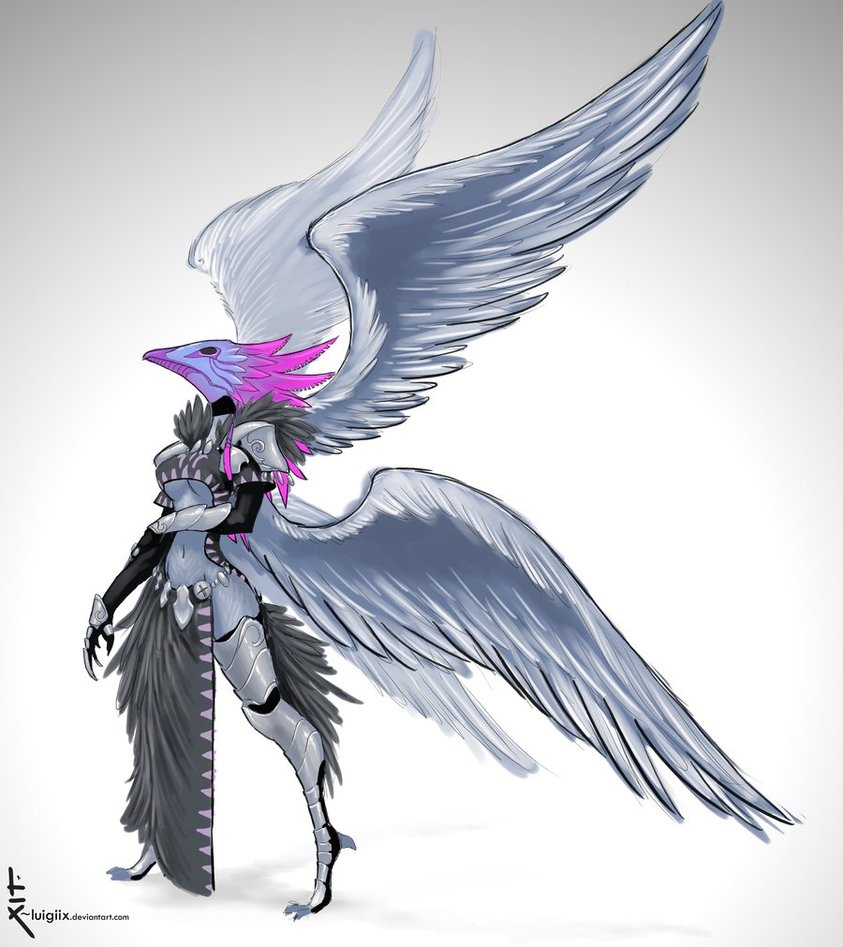
\includegraphics[width=\linewidth]{bird_race_f_concept_by_luigiix-d52w3as}

        The Ay-Matak (\textit{plural: Ay-Matakian}) are an alien species that have evolved from the birds native to their homeworld of Matak. They typically have two pairs of wings, are bi-pedal, and have two arms with opposable thumbs on each of their hands. The beak is solid and sharp at the back and sides, with the tip made out of softer material that is flexible enough to produce a variety of sounds. The male's plumage is always more colourful than the female's (which is limited to whites, greys and blacks).

        Matak, like Earth, has been lost but it was reknowned for their tall trees that almost touched the edges of the atmosphere. An overabundance of food meant that there was little need to compete for resources, and the Ay-Matak were able to indulge in the pleasures of life. The Ay-Matak place a high social value on the arts (especially those that use an abundance of colour or visual stimuli), travel, and new ideas.

        Planets under the rule of the Ay-Matak is usually formed under an Oligarchic government. The members of the government are generally influential elders who have contributed greatly to Ay-Matak culture, or have travelled far and wide in search of new ideas.

        Ay-Matak characters have the following traits:

        \begin{itemize}
            \item \textbf{Flight}: Can fly at their basic Pace and even "run" while flying. It cost 2 squares of Pace to gain 1 square of height.

            \item \textbf{Hollow-boned}: -1 toughness.

            \item \textbf{Free Edge}: Start with one free Novice Edge of their choice, regardless of requirements (except those that require other Edges).
        \end{itemize}

        \subsection{Bot/Shell}
        
        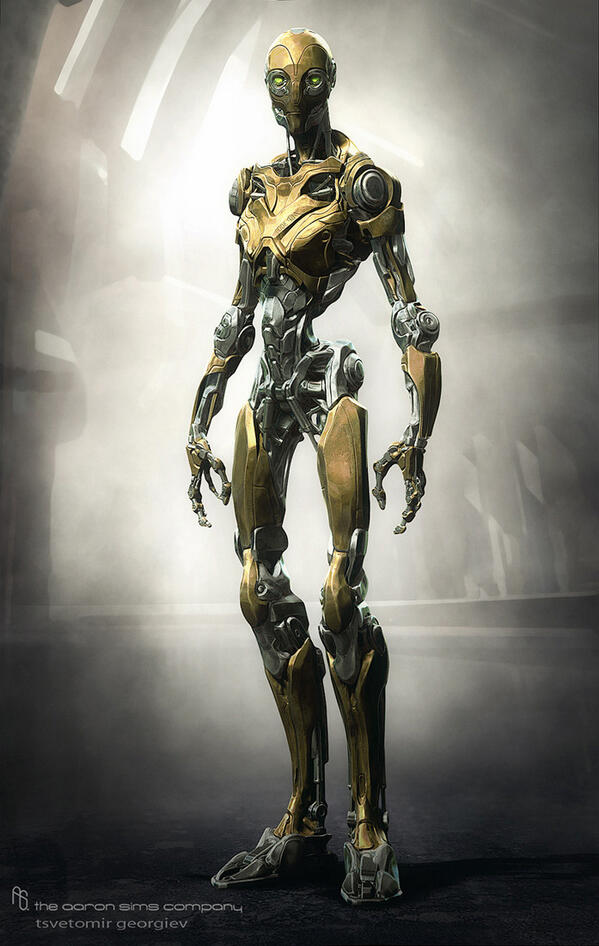
\includegraphics[width=\linewidth]{BEzZuPdCEAAgcr8.jpg}

        A common sight in any technologically-advanced society is the large number of Bots and machines performing the menial yet necessary labour. These machines are limited to a singular purpose and have a "weak AI". But technology has advanced far enough that some robots can be programmed to display human-like cognitive abilities. These Bots are considered to have "strong AI", and are usually used for highly specialised and complex work.
        
        On the other end of the spectrum are individuals who made the transition from organic to mechanical. These individuals, known as Ghosts, have chosen to digitise their conciousness and memory and upload themselves into artificial bodies known as Shells. Many in society believe that these digitised conciousnesses have lost their basic "humanity", and are indistinguishable from normal AI. 
        
        Bot and Shell characters have the following traits:
        
        \begin{itemize}
            \item \textbf{Construct}: Add +2 to recover from being Shaken, do not suffer wound modifiers, and are immune to poison and diesease. They cannot Heal naturally, and require the Repair skill to remove wounds (use like the Healing skill).

            \item \textbf{Outsider}: Organic races often mistrust and misunderstand Bots and Shells. -2 to Charisma when dealing with races other than their own.

            \item \textbf{Programming}: Start with one free d6 in one skill, representing their original programmed role.

            \item \textbf{Recharge}: Determine a power source. If you cannot access that power source at least once a day, suffer one point of Fatigue each day until incapacitated. The day after that, you go "off-line" and must be revivied with a Repair roll and a four-hour charge. This replaces the need for food and water, unless food and water is selected as the power source.
        \end{itemize}

        \subsection{Ghantak}
        
        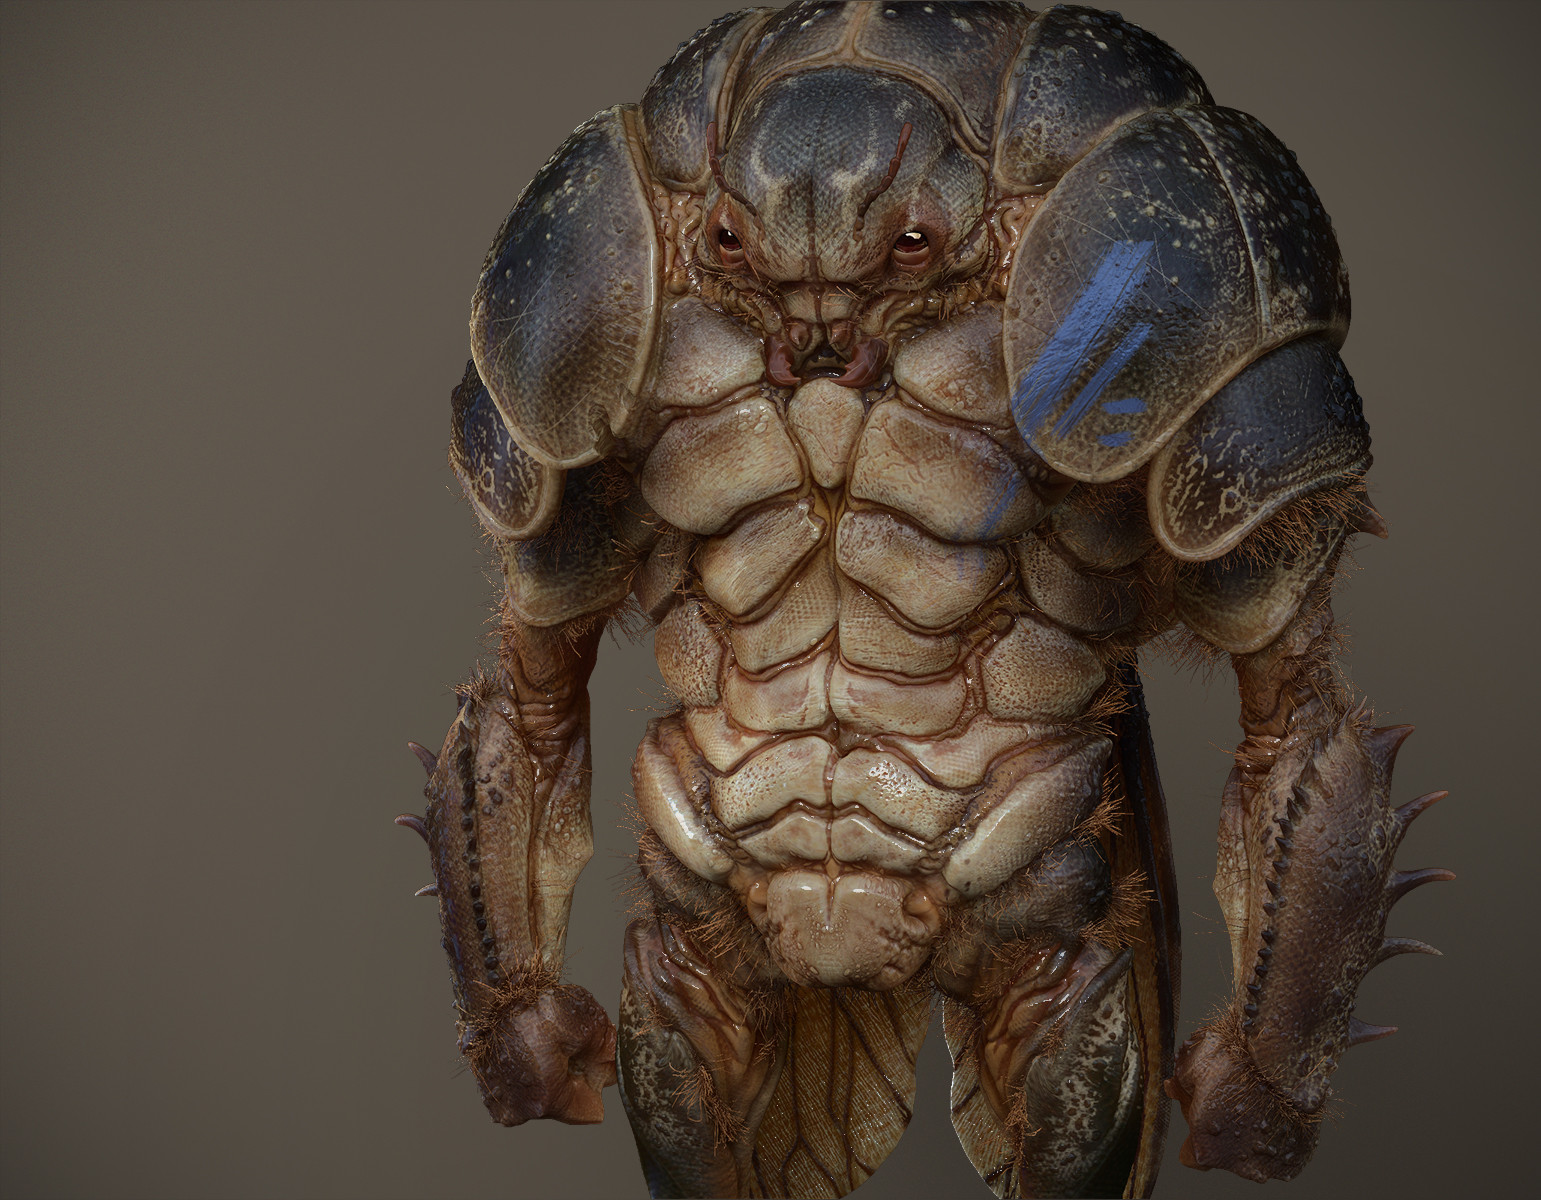
\includegraphics[width=\linewidth]{bruno-camara-beetle-brunocamara.jpg}
        
        The Ghantak (\textit{plural: Ghantakian}) are an alien species evolved from the insects native to their homeworld of Ghantak. Due to their reliance on a hive-like hierachy, the Ghantak highly value honour and tradition. Personal sacrifice for the sake of upholding Ghantakian values earns the individual glory and esteem. The race generally favours traditional solutions to problems, and individuals are uncomfortable when forced to exercise their own judgement.
        
         While there used to be multiple independant hives (each with their own Queen), the entire modern Ghantakian society is now ruled by a singular Empress. The Empress is chosen from the Queens of the remaining hives and rules until their death. This arrangement came about due to the war with the Ramollans, and has proven to be stable.
         
         Ghantakian characters have the following traits:
         
        \begin{itemize}
            \item \textbf{Carapace}: You have an armoured carapace that protects you from harm. +2 Armour.

            \item \textbf{Caste-based}: Start with one free d6 in one skill, representing your designated role in hive society.

            \item \textbf{Code of Honour}: Honor is very important to your race. You keep your word, won't abuse or kill prisoners, and generally tries to operate within the laws of the world they are on.

            \item \textbf{Reputable}: Your species is seen as dependable, loyal and predictable. +2 charisma.

            \item \textbf{Enemy of the Ramolla}: The millenia-long war between the Ramolla and Ghantak have left bitter memories. -4 Charisma when dealing with the Ramolla.
        \end{itemize}

        \subsection{Ghoa}
        
        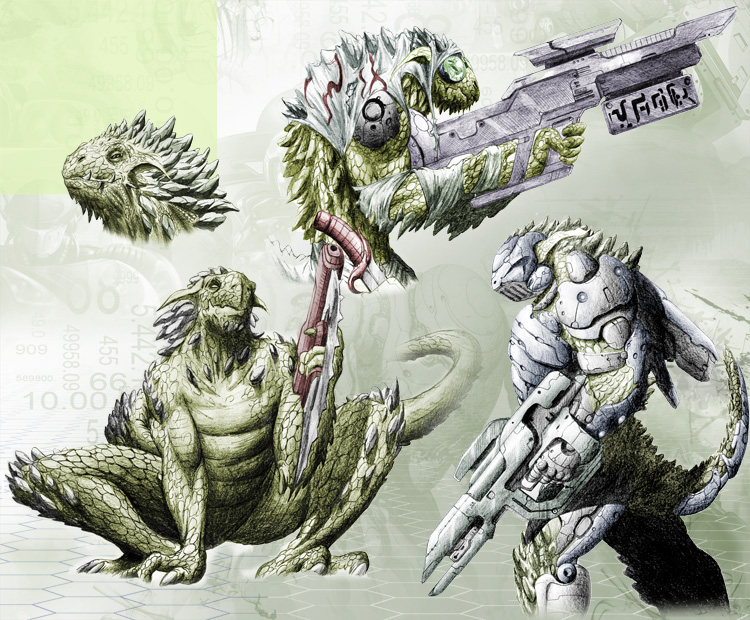
\includegraphics[width=\linewidth]{alien_reptile_concept_by_xjager513-d3ba4g7.jpg}
        
        You are an alien that has evolved from reptiles native to your planet. Your species are typically tribal, putting tribe ahead of all other social groups (including the species as a whole). Their chief mode of expression is anger, and are prone to acts of wanton violence. Disputes are traditionally resolved through force (though rarely to the death). The prospect of death rarely intimidates the Ghoa, and some actively embrace it. Their political system is based on the tribe that the Ghoa is a part of. 
        
        Ghoan characters have the following traits:
        
        \begin{itemize}
            \item \textbf{Cold Averse}: While they are not cold-blooded, the Ghoa are still uncomfortable in cold environments. Suffer -4 penalty to resist cold environment effects.
            
            \item \textbf{Ghoan Senses}: Their tongues can "taste" the air, giving them a +2 to Notice checks. (Only applies if the object or individual gives off an odour that the Ghoa can "taste")
          
            \item \textbf{Natural Weapons}: The Ghoa use their tails, claws and teeth as weapons, dealing Str+d6 damage.
          
            \item \textbf{Outsider}: Most people often distrust the fierce, angry and unblinking reptiles (their habit of eating their meat still squirming is also unsettling). -2 to Charisma when dealing with races other than their own.
            
            \item \textbf{Semi-Aquatic}: Gain a fatigue level every 15 minutes that the Ghoan holds their breath. On reaching Incapcitated, must make a Vigor roll every minute or drown. Fatigue recovers one level per 15 minutes back in air.
            
            \item \textbf{Tribal Warriors}: Their willingness to use violence to solve all problems mean that the Ghoa start with a d6 instead of a d4 in the Fighting skill.
            
        \end{itemize}

        \subsection{Human}
        
        You are a standard human, with a genetic lineage tracing all the way back to Sol.
        
        Humans have the following traits:
        
        \begin{itemize}
            \item \textbf{Free Edge}: Start with one free Novice Edge of their choice, regardless of requirements (except those that require other Edges).
        \end{itemize}

        \subsection{Ramolla}
        
        You are an alien that has evolved from the felines native to your planet. Ramollans are an extremely prideful species, and regard all other alien races as inferior to themselves. This pride drives a need to conquer and rule (both their own and other species).
        
        You have the following traits:
        
        \begin{itemize}
            \item \textbf{Agile}: Start with a d6 Agility instead of a d4.

            \item \textbf{Bloodthirsty}: Are cruel to their foes, rarely take prisoners, and feel little compunction about punishing captured foes. This causes a -4 Charisma penalty when dealing with "civilised" worlds that know of the Ramolla.

            \item \textbf{Claws}: Have retractable claws that do Str+d6 damage (and +2 to Climbing rolls).

            \item \textbf{Racial Enemy}: The millenia-long war between the Ramolla and Ghantak have left bitter memories. -4 Charisma when dealing with the Ghantak.

            \item \textbf{Low-Light vision}: Their eyes can amplify light. They can see in the dark and ignore attack penalties for Dim and Dark lighting.

            \item \textbf{Keen hearing}: +2 to notice checks that use hearing.
        \end{itemize}

        % =================
        % Attributes
        % =================

        \section{Traits}

        \subsection{Attributes}

        \begin{itemize}

            \item \textbf{Agility}: Your nimbleness, quickness and dexterity.

            \item \textbf{Smarts}: Your mental agility, how well you think on your feet, and your knowledge about the worlds that inhabit the Black.

            \item \textbf{Spirit}: Your inner wisdom and willpower.

            \item \textbf{Strength}: Your raw physical power and general fitness.

            \item \textbf{Vigor}: Your endurance, resistance to disease, and a measure of how much pain and physical damage you can shake off.

        \end{itemize}

        % =================
        % Skills
        % =================

        \subsection{Skills}

        \begin{itemize}

            \item \textbf{Athletics (Strength)}: Covers swimming, climbing and general Athletics.

            \item \textbf{Driving (Agility)}: Control ground and water vehicles.

            \item \textbf{Fighting (Agility)}: Cover all hand-to-hand (melee) attacks.

            \item \textbf{Gambling (Smarts)}: Understand the rules and odds for games of chance.

            \item \textbf{Healing (Smarts)}: Art of applying First Aid, stopping wounds and treating existing injuries. Every success and raise eliminates a wound (Healer must subtract their own wounds AND their patients wounds from the test).

            \item \textbf{Intimidation (Spirit)}: Art of frightening an opponent with sheer force of will, threats, or just really big guns.

            \item \textbf{Investigation (Smarts)}: Knows how to get information from books, computers and other media. (For getting information from people, use Streetwise).

            \item \textbf{Knowledge (Smarts)}: Knowledge skills are limited to an area of expertise. Every character has "common knowledge" where they understand their local history, etiquette, and how to operate common machinery for their tech-level. A character can take multiple Knowledge skill domains to reflect their expertise. Some available domains:
            \begin{itemize}

            \item Astrogation: Knowledge of FTL travel through Space. Required to safely plot a route through the Black and is a must for every navigator.

            \item Astronautics: Theory and practice of designing and build a spacecraft. Keeping a spacecraft flying only requires the Repair skill, but if you want to design modifications then this skill is required.

            \item Battle: Understanding of battle strategy and tactics.

            \item Computer Sciences: Covers the sciences involved in computers such as electrical, electronics, cyberware, robotics and computer theory.

            \item Language: Knowledge of a non-native language. A d4 shows that they can read, write and speak common words and phrases. A d6 can carry a halting conversation. A d8 is fluency. A d10 is mimicing dialects. A d12 is ability to recite important literary or oral works.

            \item Life Sciences: Covers the sciences about living things such asbiology, botany, ecology, exobiology, genetics, xenobiology and zoology.

            \item Material Sciences: Covers the science about non-living things such as chemistry, engineering, mathematics, mechanics and physics.

            \item Medicine: Knowledge of the latest medical theories. The Healing skill is used for actually taking care of a patient.

            \item Planetary Sciences: Covers the sciences about planets such as geology, hydrology, and meteorology.

            \item Sector Knowledge: In-depth familiarity about a particular sector that is beyond what is considered common knowledge.

            \item Social Sciences: Covers archeology, economics, law, and political science.

            \end{itemize}

            \item \textbf{Notice (Smarts)}: General alertness and ability to search for items or clues. This includes detecting ambushes, spotting hidden items, and scrutinizing people to see if they are lying or frightened.

            \item \textbf{Operations (Smarts)}: Covers all necessary skills to operate sensors, shields and other spacecraft systems.

            \item \textbf{Persuasion (Spirit)}: Art of convincing others to do what you want them to do. NPCs start in one of five different attitudes: Hostile, Uncooperative, Neutral, Friendly or Helpful. A successful roll or raise will improve their attitude, but a failure will decrease it.

            \item \textbf{Piloting (Agility)}: Control air and space vehicles.

            \item \textbf{Psionics (Smarts)}: Required for psionic characters to use their powers. For non-psionic characters, this skill represents an understanding of how psionics work.

            \item \textbf{Repair (Smarts)}: Ability to fix gadgets, vehicles, weapons, and other machines (suffer a -2 penalty if they do not have the required tools).

            \item \textbf{Riding (Agility)}: Ride and control beasts.

            \item \textbf{Security (Smarts)}: Ability to open locked locations, disarm traps, bypass alarms and hack computers. You can use this skill to protect against unwanted intruders.

            \item \textbf{Shooting (Agility)}: Covers all attempts to hit a target with a ranged weapon. Basic target number is 4 at short range.

            \item \textbf{Stealth (Agility)}: Ability to hide and move quietly, as well as palm objects and pick pockets.

            \item \textbf{Streetwise (Smarts)}: Able to gather information from the people on the street.

            \item \textbf{Survival (Smarts)}: Art of finding food, water or shelter in hostile environments.

            \item \textbf{Taunt (Smarts)}: Test of will attack against an enemy.

            \item \textbf{Throwing (Agility)}: Covers all thrown weapons such as spears and grenades.

            \item \textbf{Tracking (Smarts)}: Follow the tracks of one or more individuals in any type of terrain.

        \end{itemize}

        % =================
        % Derived Traits
        % =================

        \subsection{Derived Traits}

        \begin{itemize}

            \item \textbf{Charisma}: Your Charisma is calculated by the following formula: (Spirit / 2) - 4. It is your general likeability and manners. It is added to all persuasion and streetwise rolls.

            \item \textbf{Pace}: Your pace is calculated by the following formula: (Strength / 2) + 2. It determines how many squares of movement you can take during your turn.

            \item \textbf{Parry}: Your parry is calculated by the following formula: (Fighting / 2) + 2. Parry is the target number for melee combat or against ranged weapons within melee range.

            \item \textbf{Toughness}: Your toughness is calculated by the following formula: (Vigor / 2) + 2. You add your armour on top of toughness.

        \end{itemize}

    \end{multicols}

    \newpage

    % =================
    % Powers
    % =================

    \section{Powers}

    \begin{multicols}{2}

        Psionics have been granted special abilities due to the side-effects of TDD technology. They can manipulate matter, create fire, and some even say they can alter time. A new Psionic starts off with 3 powers at the Novice level.

        As a psionic, when you wish to cast a power you must make a Psionic skill roll. You must apply all penalties noted in the table entry, including wound and fatigue penalites. You cast the power on a success (with additional benefits on a raise), but if you fail the skill roll you cancel all currently maintained powers and you are Shaken.

        Some additional notes regarding powers:

        \begin{itemize}

            \item \textbf{Backlash}: If you roll a 1 on the Psionic skill die (regardless of the Wild Die), your power automatically fails and you suffer 2d6 damage. All sentient creatures within a Large Burst (6 diameter) centered on the Psionic also suffer 2d6 damage.

            \item \textbf{Brainburn}: If you roll a 1 on the Psionic skill die (regardless of the Wild Die), you are automatically Shaken. On a Critical Failure, you let out a psychic Surge that causes all allies within a Large Burst (6 diameter) to be Shaken as well (if they fail their Spirit roll). This can cause a wound.

            \item \textbf{Concentration}: Some powers are listed as "Concentration" and can last as long as desired. Each new power maintained inflicts a -1 to cast any new powers. Thus a Shielded Psionic can keep the power going indefinitely, but suffers a -1 penalty if they then attempt to create a Blast.

            \item \textbf{Interrupting Powers}: If a character with an activated power is Shaken or suffers a wound or Fatigue level, they must make a Smarts roll to maintain all of their powers. If the roll is failed, all powers are instantly dropped. Powers stop automatically if the psionic sleeps or is rendered unconcious.

            \item \textbf{Power Preperation}: A psionic may prepare a spell by concentrating for a round (no movement or other actions and avoid interruptions). If successful, they ignore 2 points of penalties on all powers cast with their next action. If they do not enact any powers on their next action, the preparation is lost.

        \end{itemize}

    \end{multicols}

    \subsection{Novice Powers}

    \newenvironment{powertable}{\rowcolors{2}{bgtan}{commentgreen}\longtable} {
    \endlongtable}

    \begin{powertable}{ p{.15\textwidth} p{.10\textwidth} p{.10\textwidth} p{.20\textwidth} p{.35\textwidth} }
        \hline
        \textbf{Power} & \textbf{Penalty} & \textbf{Range} & \textbf{Duration} & \textbf{Effects} \\
        Alter Light & -1 & Smarts & Concentration & Creates or negates light in a Large Burst (6 diameter) by +/-6. If the target is an opponent or item an opponent is holding, opposed by Target's agility. \\
        Attenuate & -1 & Smarts & Concentration & Sound within a Small Burst (2 diameter) is absorbed. Raise Sneak die by 1 (2 with a raise). Speaking becomes a normal action instead of Free, and you must yell to be heard. If the target is an opponent or item an opponent is holding, opposed by Target's agility. \\
        Blind & -1/-2/-3 & 12/24/48 & Instant & Target must make Agility roll at -2 to avert their gaze (-4 with raise). On a failure the target is shaken and have -2 to their Parry until their next action. On a 1, they are completely Blind and Shaken and remain Blind until they recover from being Shaken. Blinded victims suffer -6 to all Trait rolls that require vision and Parry is reduced to 2. -1 for 1 target, -2 for Medium Burst (4 diameter), -3 for Large Burst (6 diameter) \\
        Boost/Drain & -1 & Smarts & Concentration & Target gains or loses 1 die type (or 2 with raise) in a trait of your choosing (exceeding d12 by adding +1, but never lower than d4). Opposed Spirit roll, and multiple castings stack. \\
        Burst & -1 & Cone & Instant & Targets in cone suffer 2d10 damage. This counts as a heavy weapon. Cone is 9 long and 3 wide. \\
        Energy Bolt & -1 per bolt & 12/24/48 & Instant & Up to 3 bolts at 2d6 damage. Each Bolt requires it's own psionic roll and compared with target number. \\
        Deflection & -1 & Touch & Concentration & A psionic barrier that deflects incoming attacks. -2 penalty to all fighting, shooting or other attack rolls. On a raise increases the penalty to -4. Also acts as armour against area effect weapons. \\
        Fear & -1 & Smarts x 2 & Instant & All withing a Large Burst (6 diameter) must make a Fear check (at -2 with raise). Wild Cards who fail roll on the Fear table, while Extras are Panicked. \\
        Fire Bolt & -2 per bolt & 12/24/48 & Instant & Up to 3 bolts at 2d6 damage with armour piercing (AP 2). Each Bolt requires it's own psionic roll and compared with target number. \\
        Healing & -2 & Touch & Instant & Heals 1 Wound suffered within last hour, or 2 with a raise \\
        Legerdemain & 0 & Smarts & Instant & Perform a single action at range \\
        Mind Bend & -2 & Smarts & 1 round & Opposed roll vs. target's Smarts. Allows psionic to gain 1 truthful answer. On a raise, target is unaware of intrusion. \\
        Nightvision & 0 & Touch & Concentration & Half any darkness penalties (round down). On a raise, negate all darkness penalties up to the maximum of -6. \\
        Psionic Infusion & -1 & Touch & Concentration & +2 bonus to weapon damage; +4 with raise. \\
        Psionic Manipulation & 0 & Smarts x 2 & Concentration & Perform basic "tricks" with the basic elements (air, earth, fire, water). For example they can affect air to blow out candles and cool their body, open a half-meter hole in soft earth, spray sand to blind opponent (+1 to Trick roll), create a small flame, conjure up a litre of water within sight, or purify poisoned or salty water. \\
        Psionic Shield & -1 & Touch & Concentration & +2 armor; +4 with raise \\
        Restrict & -1/-2 & Smarts & Concentration & Opposed by Target's agility. Target suffers a -2 penalty to Pace, Strength and Agility checks. On a raise they are completely restrained. Affects 1 target for -1, or Medium Burst (4 diameter) for -2 (use penalty for concentration). \\
        Soothe & 0 & Touch & Instant & Removes 1 Fatigue level (2 with raise), and restores conciousness. Can remove Shaken status. \\
        Speed & 0 & Touch & Concentration & Basic Pace is doubled, and running is free action with raise. \\
        Stun & -1 & 12/24/48 & Special & All targets in Medium Burst (4 diameter) must roll Vigor (-2 with raise) or be Shaken \\
        Wall Walker & -1 & Touch & Concentration & Move on any surface at half Pace, or full Pace with raise \\
    \end{powertable}

    \newpage

    % =================
    % Terminology
    % =================

    \section{Terminology}

    \begin{multicols}{2}

        \begin{itemize}

            \item \textbf{AGI}: Artificial General Intelligence or "\textit{strong AI}". An AI that has cognitive faculties comparable to a human or higher.

            \item \textbf{AI}: Artificial Intelligence. Generally used for "\textit{weak AI}", or specialised AI that do not encompass the full range human-level cognitive abilities.

            \item \textbf{AR}: Augmented Reality. Information that is overlaid onto your real-world senses. AR data is usually entoptic (visual), but can also be audio, tactile, olfactory, kinesthetic (body awareness), emotional, and other senses.

            \item \textbf{Ay-Matak}: Alien race that has evolved from birds native to their planet. The species have an innate wanderlust, and are never happy staying in one place too long. They place high social value in the areas of art, pleasure and excitement. Their political system is based on oligarchic rule by influential elders.

            \item \textbf{Black}: Slang term for space.

            \item \textbf{Bots}: Robots.

            \item \textbf{Cortical Stack}: An implanted electronic data storage used for memory and personality backups. Located where the spine meets the skull.

            \item \textbf{Cradle}: Slang term for Earth. Location is currently unknown.

            \item \textbf{Credit}: Standard interchangeable monetary unit accepted by most space-faring worlds. Issued as either electronic banking entries, or embedded onto physical electronic chips. Some primitive worlds use "notes" made of plastic or paper.

            \item \textbf{Cyberware}: Generic term for the neural interface technology that melds metal and flesh into a coherent whole. This technology enables AR, Cortical Stacks, Ghosts in their Shells, and Sim-Sense.

            \item \textbf{ECM}: Electronic Counter Measures. A suit of electronic tools designed to target and cripple enemy sensors to make you almost impossible to track and hit.

            \item \textbf{Entoptics}: AR images that you "see" in your head ("Entoptic" means "within the eye").

            \item \textbf{FTL}: Faster-Than-Light.

            \item \textbf{Ghantak}: Alien species that have evolved from insects native to their planet. The species place a high value on honour and tradition, with a singular Queen ruling over the entire species. Personal sacrifice for the sake of upholding Ghantakian values earns you glory and esteem. The race favours traditional solutions to problems, and individuals are uncomfortable when forced to exercise their own judgement.

            \item \textbf{Ghoa}: Alien species that have evolved from reptiles native to their planet. The species are typically tribal, putting their tribe ahead of all other social groups (including the species as a whole). Their chief mode of expression is anger, and the Ghoa are prone to acts of wanton violence. Disputes are traditionally resolved through force, sometimes but rarely to the death. The prospect of death rarely intimidates the Ghoa, and some even actively embrace it. Their political system is based entirely upon the tribe that the Ghoa is a part of.

            \item \textbf{Ghost}: Slang term used for a digitised persona. Some individuals have used Cortical Stacks to make a digital copy of themselves. These copies exist on digital hardware or in artifical bodies known as Shells. There is debate on whether these copies are really "people" or just another AGI.

            \item \textbf{IDD}: Intra-Dimensional Drive. Spaceship engine used to achieve FTL speeds based on TDD technology. To guard against another Surge-like event, IDD only manipulates Space-Time within a precisely defined spectrum. TDD does not have this limitation, and therefore TDD technology is vastly superior in performance and achievable FTL speeds.

            \item \textbf{Jump Portal}: Large gateways that used TDD technology to allow large cargo ships to travel at FTL speeds. All known portals are currently defective and inoperable.

            \item \textbf{Muse}: Slang for personal AI helper programs.

            \item \textbf{Psionic}: An individual adversely affected by trans-dimensional energy. Some have been granted the ability to manipulate Space-Time, while others become malformed and driven mad. Also known as psychics, paranorms, and jsingshen.

            \item \textbf{Propulsion Thruster}: Conventional spacecraft engine that propels energy away from the spacecraft to create thrust. Used for interplanetary travel within a star system.

            \item \textbf{Reclaimers}: Euphemistic slang for scavengers. These individuals search and scour the Black for salvageable ruins.

            \item \textbf{Shell}: Slang term for an artificial body. These bodies can either be synthetic or biological. There is debate on whether these Shells are really "people" or just another Bot.

            \item \textbf{Sim-sense}: Experiencing someone else's sensory input (in real-time or recorded).

            \item \textbf{Space-Time}: The concepts of time and three-dimensional space fused in a four-dimensional continuum.

            \item \textbf{Splicer}: Slang for an individual that has undergone extensive genetic modification and transformation.

            \item \textbf{Surge}: A mysterious event that overloaded all technology that utilised trans-dimensional energy.

            \item \textbf{TDD}: Trans-Dimensional Drive. Heavy utilised technology that bends Space-Time to achieve FTL travel. A side effect is the creation of psionics.

            \item \textbf{Tech-Level}: Standard technology classification for worlds. There are seven tech-levels, ranging from 0 (stone-age) to 6 (advanced technology exceeding anything from pre-Surge civilisation)

            \item \textbf{Trans-dimensional energy}: A form of energy that is the by-product of manipulating the multiple dimensions of Space-Time by collapsing and bending it. Not much is known about this energy.

            \item \textbf{Uplifted}: Animals that are biologically and geneticatlly engineered to have higher intelligence and sentience.

            \item \textbf{Xenomorph}: Alien life form.

        \end{itemize}

    \end{multicols}

\end{document}
